% MadNLP4NN.jl Technical Report (Intermediate)
% This document summarizes the formulation, design choices, and implementation details
% of the MadNLP4NN.jl framework.

\documentclass[11pt]{article}
\usepackage[margin=1in]{geometry}
\usepackage{amsmath, amssymb, amsthm}
\usepackage{mathtools}
\usepackage{hyperref}
\usepackage{graphicx}
\usepackage{booktabs}
\usepackage{microtype}
\usepackage{enumitem}
\usepackage{xcolor}

\hypersetup{
  colorlinks=true,
  linkcolor=[rgb]{0.1,0.2,0.6},
  citecolor=[rgb]{0.1,0.5,0.1},
  urlcolor=[rgb]{0.1,0.2,0.6}
}

\title{MadNLP4NN.jl: A Toy-Level Technical Report on Reduced-Space NLP with Neural Networks and GPU-Accelerated Solvers}
\author{Hongxuan Liu}
\date{\today}

\begin{document}

\maketitle

\begin{abstract}
We present MadNLP4NN.jl, a Julia/Python framework for solving constrained optimization problems involving trained neural networks. The framework uses a reduced-space nonlinear programming (NLP) formulation, solved with the interior-point solver MadNLP (Shin et al.), which keeps the optimization problem size independent of the neural network's internal complexity. It features dual backends for network evaluation and automatic differentiation (AD): a pure-Julia backend using Flux with Zygote (Innes) and a Python backend using JAX with JIT compilation (Bradbury et al.), both callable from a unified Julia interface. We detail the implementation, including modular objectives, a smooth ReLU approximation, and a comprehensive training pipeline for generating models (MLPs, ResMLPs) and using pre-trained ResNets. We motivate our design choices, particularly the reduced-space formulation over full-space alternatives, and analyze the performance trade-offs. Future work will focus on systematic GPU benchmarking, batched multi-start optimization on projected non-convex landscapes, scaling to larger models and decision spaces on scalable GPU systems, and implementing advanced second-order approximations like Hessian-vector products.
\end{abstract}

\section{Introduction}
Solving large-scale constrained optimization problems and training/evaluating modern neural networks both benefit significantly from GPU acceleration. On the optimization side, second-order interior-point methods implemented in solvers such as MadNLP have demonstrated high performance on GPUs (Shin et al.). On the machine learning side, mature ecosystems such as PyTorch, JAX, and Flux/Zygote exploit the highly parallel structure of matrix–vector operations (Paszke et al.; Bradbury et al.; Innes).

In many industrial and scientific applications, optimization and machine learning naturally intersect. Representative examples include:
\begin{itemize}[leftmargin=1.5em]
  \item \textbf{Decision optimization with learned surrogates}: surrogate models (e.g., neural networks) approximate expensive physical simulators, enabling fast optimization under constraints.
  \item \textbf{Safe control and planning}: neural policies or dynamics models appear inside constraints or objectives; safety envelopes and reachability margins induce nonlinear constraints.
  \item \textbf{Design and inverse problems}: neural networks map designs to performance metrics, while the optimizer searches feasible designs meeting targets.
  \item \textbf{Robustness and verification}: adversarial or worst-case inputs are obtained by optimizing against a trained classifier/regressor subject to norm or domain constraints. Mixed-integer formulations and modeling toolkits such as OMLT offer exact treatments for piecewise-linear operators (Tsay et al.) but do not align with smooth second-order methods.
\end{itemize}

\paragraph{Research gap.} Despite this natural synergy, practical pipelines often keep optimization and ML in disjoint stacks: classical NLP solvers execute primarily on CPUs, while ML frameworks run on GPUs. Recent progress shows promise in both \emph{optimization on GPUs} (e.g., MadNLP, ExaModels, cuPDLP/\texttt{cuPDLPx.jl}; Shin et al.; Pacaud et al.; Lu et al.) and \emph{optimization with neural networks}. However, existing implementations frequently split computation between CPU-based optimization and GPU-based neural network derivatives, leading to CPU–GPU data-transfer bottlenecks that become prohibitive for modern, large neural networks.

\paragraph{Our contribution.} MadNLP4NN.jl provides a unified framework that:
\begin{itemize}[leftmargin=1.5em]
  \item Implements a \textbf{reduced-space} NLP formulation, where the neural network is a black-box function, keeping the KKT system size independent of network complexity (Shin et al.; Pacaud et al.).
  \item Provides \textbf{dual, high-performance AD backends}: (1) a pure-Julia backend using Flux with Zygote's reverse-mode AD (Innes), and (2) a Python backend using JAX with its JIT compilation (Bradbury et al.), both callable from a unified Julia interface.
  \item Exploits problem structure by using fast paths for linear and quadratic constraints within the Hessian callbacks to improve solver efficiency.
  \item Includes a comprehensive Python-based pipeline for \textbf{model generation}, featuring synthetic datasets, hyperparameter search with Optuna (Akiba et al.), and training for multiple architectures (MLPs, ResMLPs).
  \item Integrates seamlessly with \textbf{MadNLP}'s advanced features, including its portfolio of sparse linear solvers and readiness for GPU acceleration.
\end{itemize}
This design reduces CPU–GPU data movement, preserves flexibility across diverse network architectures (including MLPs, ResMLPs, and ResNets), and provides a scalable foundation for solving complex optimization problems with integrated machine learning models. We conclude by discussing promising future directions, including systematic GPU benchmarking, batched multi-start optimization, scaling to larger problems and models on distributed systems, and implementing advanced second-order approximations.

\section{Methodology}
\subsection{Problem formulation}
We consider constrained problems of the form
\begin{equation}
  \label{eq:base}
  \min_{x \in \mathbb{R}^n} \; f\big(x, \theta\big) \quad \text{s.t.} \quad g(x) \le 0,
\end{equation}
where $x$ denotes decision variables, $\theta$ are fixed neural network parameters obtained from training, $f$ is an objective that depends on the neural network outputs and possibly regularization terms, and $g$ encodes constraints such as elementwise bounds (box constraints) or norm constraints (spherical constraints). Typical objectives include squared distance to a target output, optionally combined with quadratic regularization $\lVert x - x_0 \rVert^2$.

\subsection{Full-space formulation}
In a full-space scheme, the neural network computation is \emph{embedded explicitly} as constraints layer-by-layer. Let $z^{(\ell)}$ be the pre- or post-activation at layer $\ell$. A feed-forward MLP with ReLU activations can be written as
\begin{align}
  z^{(1)} &= W^{(1)} x + b^{(1)}, \\
  a^{(1)} &= \phi\big(z^{(1)}\big), \\
  z^{(2)} &= W^{(2)} a^{(1)} + b^{(2)}, \\
          &\;\vdots \\
  y &= W^{(L)} a^{(L-1)} + b^{(L)},
\end{align}
with constraints enforcing $a^{(\ell)} = \phi(z^{(\ell)})$ for each hidden layer and $\phi$ the activation (e.g., ReLU). The NLP therefore introduces all intermediate variables $\{z^{(\ell)}, a^{(\ell)}\}_{\ell=1}^{L-1}$ and equalities that mirror the network computation.

While conceptually straightforward, this approach is impractical for modern networks for several reasons:
\begin{enumerate}[leftmargin=1.5em]
  \item \textbf{KKT system scaling.} The number of variables and constraints grows linearly with network depth and width. The KKT system size therefore scales with the neural network, making factorization intractable for state-of-the-art models. Memory footprints can reach hundreds of megabytes or more.
  \item \textbf{Loss of optimized kernels.} By re-implementing forward/AD computations inside the NLP, we forgo highly optimized ML library kernels (e.g., JAX, Flux, PyTorch) that exploit fused operations, tensor cores, and layout-specific optimizations.
  \item \textbf{Poor robustness across architectures.} Any architectural change (residual connections, convolutions, normalization layers) requires re-deriving constraints and often bespoke modeling work, increasing maintenance burden and limiting experimentation.
\end{enumerate}

\subsection{Reduced-space formulation}
MadNLP4NN.jl adopts a reduced-space strategy where the neural network is treated as an encapsulated, differentiable map whose internal computations do not expand the NLP's variable space. Let the network $\mathcal{N}_\theta: \mathbb{R}^n \to \mathbb{R}^m$ be defined by a composition of layer functions:
\begin{equation}
  \mathcal{N}_\theta(x) = (L_k \circ \phi \circ L_{k-1} \circ \dots \circ \phi \circ L_1)(x),
\end{equation}
where $L_i(y) = W_i y + b_i$ and $\phi$ is a smooth activation function. In the reduced-space formulation, this entire computation is treated as a ``black-box'' function call. The NLP is defined only in terms of the input $x$ and the final output $y = \mathcal{N}_\theta(x)$:
\begin{equation}
  \min_{x \in \mathbb{R}^n} \quad f(x, \mathcal{N}_\theta(x)) \quad \text{s.t.} \quad g(x) \le 0.
\end{equation}
The objective $f$ (e.g., squared distance) and its derivatives are evaluated by first computing $\mathcal{N}_\theta(x)$ and then applying the chain rule, with derivatives of $\mathcal{N}_\theta$ provided by an external AD engine (JAX or Zygote). This enables:
\begin{itemize}[leftmargin=1.5em]
  \item \textbf{Scalability}: the KKT system size depends only on $n$, not on network parameters;
  \item \textbf{Performance}: reuse of optimized ML kernels and JIT compilation for derivatives;
  \item \textbf{Flexibility}: architecture changes require no NLP reformulation.
\end{itemize}
This approach cleanly separates the concerns of the optimizer (which operates on $x$) and the neural network evaluator (which handles the complex internal computations).

\subsection{Handling non-differentiable ReLU}
ReLU is ubiquitous in large-scale neural networks due to its simplicity, mitigation of vanishing gradients on plateaus, and favorable optimization behavior. However, ReLU is non-differentiable at zero, which is problematic for second-order methods that require Hessians.

MadNLP4NN.jl employs a \textbf{smooth ReLU} (softplus) approximation:
\begin{equation}
  \label{eq:smooth-relu}
  \operatorname{smooth\_relu}(x; \alpha) \;=\; \alpha\, \log\big(1 + e^{x/\alpha}\big), \quad \alpha > 0,
\end{equation}
with small $\alpha$ (default $10^{-3}$) yielding a close approximation to ReLU while ensuring $C^\infty$ smoothness. This enables consistent gradient and Hessian computations across Flux/ForwardDiff, Flux/Zygote, and JAX backends. The choice is motivated by:
\begin{itemize}[leftmargin=1.5em]
  \item \textbf{Numerical stability}: softplus is well-conditioned and widely used in ML libraries;
  \item \textbf{Implementation simplicity}: drop-in replacement for ReLU in forward graphs;
  \item \textbf{Compatibility}: consistent behavior across Julia and Python stacks.
\end{itemize}

\paragraph{Alternatives.} Several alternatives may be considered depending on application needs:
\begin{itemize}[leftmargin=1.5em]
  \item \emph{Piecewise-smooth homotopy}: start with a smooth surrogate and gradually decrease $\alpha$ to approach ReLU; 
  \item \emph{Squared ReLU or GELU variants}: maintain smoothness while preserving ReLU-like sparsity patterns;
  \item \emph{Mixed-integer formulations}: exact modeling of ReLU (as in MILP/MINLP toolkits) via big-M or convex hulls---accurate but incompatible with second-order continuous solvers and often intractable at scale; see OMLT (Tsay et al.).
\end{itemize}
Our framework focuses on smooth surrogates to leverage continuous second-order methods and GPU-accelerated linear algebra.

\section{Experimental Setup and Implementation}
This section details the optimization tasks, datasets and models, training and acquisition of pre-trained networks, evaluation backends and AD implementations, and solver configurations, with direct references to the implementation in this repository. We emphasize design decisions that improve numerical robustness, scalability, and solver efficiency.

\subsection{Task specification (objectives and constraints)}
Our primary task is to \emph{reconstruct an input} $x$ whose network output matches a target vector $t$ (targeted class or desired activation pattern). The canonical objective in our implementation is the squared distance, exposed as \texttt{NeuralNetworkObjective} (see \texttt{src/nlp\_interface.jl}):
\begin{equation}
  \min_{x \in \mathbb{R}^n} \; \underbrace{\big\lVert \mathcal{N}_\theta(x) - t \big\rVert^2}_{\texttt{target\_distance}} \quad \text{s.t.} \quad g(x) \le 0.
\end{equation}

Beyond pure target matching, we often want to restrict the search to a plausible region around a reference $x_0$ (e.g., an existing sample or an initialization). Our \texttt{QuadraticRegularization} module implements a Tikhonov-style penalty with weight $\lambda$ (see \texttt{src/nlp\_interface.jl}):
\begin{equation}
  \min_{x} \; \big\lVert \mathcal{N}_\theta(x) - t \big\rVert^2 \; + \; \lambda\, \lVert x - x_0 \rVert^2, \qquad \lambda \ge 0.
\end{equation}
This objective supports two common use cases: (i) \emph{plausibility}---encouraging proximity to a known data manifold; (ii) \emph{solver stability}---controlling trust-region size to reduce ill-conditioning. Arbitrary composite objectives are supported via \texttt{CompositeObjective}, enabling custom user-defined addenda.

Constraints are modular and reflect the design of \texttt{BoxConstraints}, \texttt{SphericalConstraint}, and \texttt{CompositeConstraint} (see \texttt{src/nlp\_interface.jl}):
\begin{align}
  \text{Box:}\qquad &x - x_{\max} \le 0,\qquad x_{\min} - x \le 0, \\
  \text{Spherical:}\qquad &\lVert x - x_0 \rVert^2 - R^2 \le 0.
\end{align}
Implementation details are leveraged in our callbacks (\texttt{src/nlp\_model.jl}).

\subsection{Pre-trained model training and acquisition}
We evaluate two avenues for obtaining models, directly mirrored by our code paths:
\begin{itemize}[leftmargin=1.5em]
  \item \textbf{In-house training}, orchestrated from Julia via PythonCall: see \texttt{src/python\_interface.jl}, invoking \texttt{python/main.py} and \texttt{python/trainer.py}. We support synthetic (Gaussian Mixture, Nonlinear Manifold) and real datasets (MNIST, FashionMNIST, CIFAR-10).
  \item \textbf{Acquired pre-trained models} for CIFAR-10 ResNet variants (20/32/44/56 layers), consumed by the JAX evaluator (\texttt{python/jax\_nn\_evaluator.py}) and referenced under 
  \\\texttt{output/models\_ablation/cifar/}.
\end{itemize}

\paragraph{Synthetic datasets.} Implementations reside in \texttt{python/dataset\_constructor.py}, with explicit parameterization and on-disk layout.
\begin{itemize}[leftmargin=1.5em]
  \item \emph{Gaussian Mixture (GM)}: For each class $c \in \{1,\dots,C\}$, we sample $N/C$ points from a mixture of $n_{\text{comp}}$ diagonal Gaussians. Each component has a random mean $\mu_{c,k} \sim \mathcal{N}(0,4I)$ and diagonal scales $\sigma_{c,k}$ drawn log-normally (\texttt{scale = exp(randn()*0.5)} per coordinate). We then assemble class-wise batches and normalize the aggregate data to $[0,1]$. Controlled by $(N, d, C, n_{\text{comp}})$ and seeded for reproducibility.
  \item \emph{Nonlinear Manifold (NM)}: We draw latent $z \in \mathbb{R}^{m}$, linearly project via a random matrix to $\mathbb{R}^{d}$, and add nonlinearity depending on \texttt{nonlinearity} $\in$ \{polynomial, trigonometric, mixed\}. For example, polynomial adds quadratic and cubic terms; trigonometric applies sinusoidal transforms; mixed combines both. Each class receives a random shift to increase inter-class separation. Data is normalized to $[0,1]$. Parameters: $(N, d\!=\!\texttt{ambient\_dim}, m\!=\!\texttt{manifold\_dim}, C, \texttt{nonlinearity})$.
\end{itemize}
Naming convention and storage: GM uses \texttt{GM\_n\{N\}\_d\{d\}\_c\{C\}\_comp\{K\}\_s\{seed\}}, NM uses \\\texttt{NM\_n\{N\}\_a\{d\}\_m\{m\}\_c\{C\}\_\{nonlin\}\_s\{seed\}}. We persist \texttt{data.pt}, \texttt{labels.pt}, and \texttt{metadata.json} under \texttt{output/datasets/\{type\}/\{name\}}. This design enables generating arbitrarily many labeled samples and reproducing training/evaluation splits precisely.

\paragraph{Real datasets.} MNIST and FashionMNIST (28$\times$28 grayscale, flattened to $d=784$ when \texttt{flatten=true}), and CIFAR-10 (32$\times$32 RGB, flattened to $d=3072$ for MLP/ResMLP; CNNs use $(3,32,32)$). We split train/val 80/20 (\texttt{random\_split}), shuffle train batches, and serialize dataset metadata for downstream consumers.

\paragraph{Model families and configurations.} For in-house models we use MLP and ResMLP (see \texttt{python/neural\_network.py}). Parameter counts are deterministic given $(d, C, \texttt{hidden\_dims})$ and can be computed analytically. MAdds, which approximate the number of multiply-add operations per forward pass, also scale predictably. For MLPs, the computational cost is dominated by the first layer's matrix-vector product, scaling linearly with the input dimension $d$. We report example values for models with $d=784$ and $C=10$.
\begin{table}[h!]
\centering
\caption{MLP/ResMLP configurations at $d=784$, $C=10$. MAdds approximate multiply-adds per forward pass.}
\begin{tabular}{@{}lrrrr@{}}
\toprule
Model & Hidden structure & Params & MAdds ($est.$) & Notes \\
\midrule
small\_mlp & [128, 64] & 0.109M & 0.109M & dropout optional \\
medium\_mlp & [256, 128, 64] & 0.243M & 0.243M &  \\
large\_mlp & [512, 256, 128, 64] & 0.575M & 0.575M &  \\
small\_resmlp & $h$=128, $B$=2 & 0.168M & 0.167M & two $h\times h$ per block \\
medium\_resmlp & $h$=256, $B$=4 & 0.730M & 0.728M &  \\
large\_resmlp & $h$=512, $B$=6 & 3.56M & 3.55M &  \\
\bottomrule
\end{tabular}
\end{table}

For acquired CIFAR-10 CNNs we use standard ResNet variants (parameters typical for CIFAR implementations). Our JAX evaluator reconstructs forward passes directly from PyTorch \texttt{state\_dict}, including custom conv/batchnorm/pooling implemented in \texttt{jax\_nn\_evaluator.py} (see \_conv2d\_jax, \_batchnorm\_jax, etc.).
\begin{table}[h!]
\centering
\caption{CIFAR-10 ResNet family (typical figures; may vary by implementation).}
\begin{tabular}{@{}lrr@{}}
\toprule
Model & Params & MAdds ($est.$) \\
\midrule
ResNet-20 & 0.27M & 41M \\
ResNet-32 & 0.46M & 69M \\
ResNet-44 & 0.66M & 97M \\
ResNet-56 & 0.85M & 125M \\
\bottomrule
\end{tabular}
\end{table}

\paragraph{Training pipeline and hyperparameters.} Training and hyperparameter search are defined in \texttt{python/main.py} and \texttt{python/trainer.py} and are driven from Julia via \texttt{src/python\_interface.jl}.
\begin{itemize}[leftmargin=1.5em]
  \item \emph{Data loaders}: 80/20 train/val split (seeded); \texttt{batch\_size} default 64; \texttt{num\_workers}=0 for portability.
  \item \emph{Loss/optimizers}: cross-entropy loss; Adam/AdamW/SGD considered with tunable \texttt{weight\_decay}.
  \item \emph{Hyperparameter search} (Optuna): $\texttt{learning\_rate} \in [10^{-4},10^{-2}]$ (log-scale), $\texttt{weight\_decay} \in [10^{-6},10^{-3}]$ (log-scale), $\texttt{optimizer} \in \{\text{adam, adamw, sgd}\}$. Trials default to 50; each trial trains for \texttt{hparam\_search\_epochs} (default 20). Objective is best validation accuracy.
  \item \emph{Final training}: retrain from scratch with best hyperparameters for \texttt{epochs} (default 100) using a cosine annealing LR scheduler.
  \item \emph{Artifacts}: models saved to \texttt{output/models/\{dataset\_name\}/\{model\_config\}/model\_seed\{seed\}.pt} with \texttt{model\_config}, \texttt{train\_args}, and training \texttt{history}. A \texttt{results\_seed\{seed\}.json} summarizes metrics.
\end{itemize}

\paragraph{Input/output dimensions.} For all classification tasks we use $C=10$ classes with one-hot targets. Input dimensions by dataset:
\begin{itemize}[leftmargin=1.5em]
  \item MNIST/FashionMNIST: $d=784$ (flattened 28$\times$28) for MLP/ResMLP; CNNs can consume $(1,28,28)$.
  \item CIFAR-10: $d=3072$ (flattened 32$\times$32$\times$3) for MLP/ResMLP; CNNs consume $(3,32,32)$.
  \item GM: user-specified $d$ (default 784), $C=10$, $K=n_{\text{comp}}$ per class.
  \item NM: $d=\texttt{ambient\_dim}$ (default 784), $m=\texttt{manifold\_dim}$ (default 50), $C=10$.
\end{itemize}
Crucially, the KKT system dimension depends only on $n=d$ (the decision space) and is \emph{independent} of the network parameter count, underscoring the scalability advantage of the reduced-space approach.

\subsection{Test machine and software stack}
Experiments were run CPU-only on an Apple M3 Max platform, with the following software stack matching \texttt{Project.toml} and \texttt{python/requirements.txt}:
\begin{itemize}[leftmargin=1.5em]
  \item Julia 1.9; Python 3.10
  \item PyTorch $\ge$ 2.0, torchvision, Optuna; JAX/JAXLIB $\ge$ 0.4
  \item MadNLP (0.7), NLPModels (0.20), Flux (0.14), ForwardDiff (0.10), Zygote (0.6)
  \item Optional GPU packages (MadNLPGPU, MadNLPHSL) were \emph{not} used for the CPU-only runs.
\end{itemize}
We report CPU-only results. GPU-enabled solvers and JAX acceleration are supported by the framework and recommended for larger problems.

\subsection{Automatic differentiation implementations}
\paragraph{Python/JAX backend.} The JAX evaluator (\texttt{python/jax\_nn\_evaluator.py}) loads PyTorch checkpoints into JAX functions for MLP/ResMLP and ResNet. JAX is well-suited for scalable ML+Opt due to its function-oriented design, strong JIT compiler, and first-class GPU/TPU support. Key implementation points:
\begin{itemize}[leftmargin=1.5em]
  \item \textbf{Model import}: \texttt{load\_pytorch\_model\_to\_jax} inspects \texttt{state\_dict} to infer architecture and constructs JAX forward functions.
  \item \textbf{JIT}: The forward pass is JIT-compiled (\texttt{self.jax\_forward\_jit}), amortizing overhead.
  \item \textbf{Derivatives}: We build closures (via \texttt{functools.partial}) that bind parameters/targets/etc. so that JAX \texttt{grad/jacobian/hessian} act on $x$ alone.
\end{itemize}
The evaluator exposes: \texttt{evaluate\_obj(x)}, \texttt{evaluate\_grad(x)}, \texttt{evaluate\_cons(x)}, \texttt{evaluate\_jac(x)}, and \texttt{evaluate\_hess(x,y)} for the Lagrangian.

\paragraph{Julia/Flux backend.} In \texttt{src/nlp\_model.jl}, we use Flux for modeling with Zygote or ForwardDiff for AD.
\begin{itemize}[leftmargin=1.5em]
  \item \textbf{Zygote (Default)}: This modern reverse-mode AD is the default and vastly more efficient for our tasks. For gradients, we use \texttt{Zygote.gradient}. For Hessians, we apply a forward-over-reverse strategy by taking the ForwardDiff Jacobian of the Zygote gradient function.
  \item \textbf{ForwardDiff}: While available, forward-mode AD is less efficient for functions $\mathbb{R}^n \to \mathbb{R}$ when $n$ is large. It is mainly kept for baseline comparisons and small-scale problems. In our tests, Zygote consistently shows speedups of 10--100$\times$ over ForwardDiff.
\end{itemize}
While Julia's ML/AD ecosystem is rapidly maturing, Python's is more developed. However, the Flux backend avoids Python interop overhead during solver callbacks.

\subsection{MadNLP solver settings}
MadNLP solves the NLP by calling back to our \texttt{NeuralNetworkNLPModel} for function and derivative evaluations via the NLPModels.jl interface (\texttt{obj}, \texttt{grad!}, \texttt{cons!}, \texttt{jac\_coord!}, \texttt{hess\_coord!}). Configurable options (see \texttt{run\_opt\_ablation.jl}) include:
\begin{itemize}[leftmargin=1.5em]
  \item \textbf{KKT systems}: \texttt{SparseKKTSystem} (default), with dense/condensed variants available.
  \item \textbf{Linear solvers}: A wide portfolio including Umfpack, Lapack, MUMPS (used in ablations), Pardiso, and various HSL routines for CPU. On GPU, MadNLPGPU provides cuDSS, cuSOLVER, and others.
  \item \textbf{Performance}: \texttt{blas\_num\_threads} (also sets \texttt{OMP\_NUM\_THREADS}), \texttt{max\_iter}, \texttt{tol}, and \\\texttt{disable\_garbage\_collector}.
\end{itemize}
Our CPU runs primarily use \texttt{SparseKKTSystem} with MUMPS. Both the JAX and Flux backends implement box constraints as explicit linear inequalities in the callback functions, ensuring their Hessian contribution is zero. This improves KKT system sparsity and linear solver performance.

\section{Experimental Results}

\subsection{Experimental settings}
We follow the experimental protocol implemented in \texttt{examples/run\_opt\_ablation.jl}. The design emphasizes comparability across models and backends while producing stable aggregate statistics.
\begin{enumerate}[leftmargin=1.5em]
  \item \textbf{ML training task selection.} We report results for six MNIST models we trained in-house (small/medium/large MLPs and small/medium/large ResMLPs), and for externally acquired CIFAR-10 ResNet models. Synthetic datasets (Gaussian Mixture, Nonlinear Manifold) yielded models that fit extremely well (suggesting intrinsic dimensionality far below the VC dimension of the models), potentially masking the complexity of the downstream optimization task; thus, we prioritized MNIST for in-house models. For CIFAR-10, MLP/ResMLP lacked the inductive bias to train satisfactorily (validation loss plateaued), so we adopted pre-trained ResNets.
  \item \textbf{Seeds, targets, and averaging.} For each model, we fixed 10 random initial points (one per target class) and, for each initial point $i$, optimized toward the one-hot target vectors for classes $i$. This yields robust averages across both random initializations and target classes.
  \item \textbf{Optimization and solver parameters.} Unless otherwise specified, we used: \texttt{max\_iter} = 1000, \texttt{tol} = $10^{-4}$, \texttt{print\_level} = ERROR, \texttt{device} = CPU, \texttt{kkt\_system} = SparseKKTSystem, \texttt{linear\_solver} = MUMPS, \texttt{blas\_num\_threads} = 8, \texttt{disable\_garbage\_collector} as configured in the script. Random seed was 42 in Julia and mirrored in Python (NumPy, random) for the JAX backend. See \texttt{examples/run\_opt\_ablation.jl} for the authoritative configuration.
  \item \textbf{Constraint representation.} In both the JAX and Flux implementations, box constraints are encoded as linear inequalities within callbacks (zero Hessian contribution), which reduces fill-in in the Lagrangian Hessian and improves KKT compactness. Spherical constraints are quadratic and contribute a constant Hessian term (scaled identity) in the Lagrangian.
  \item \textbf{Timing and accounting.} For each optimization run, we report total solve time, internal MadNLP time (solve time minus evaluation time), total evaluation time, and their percentages. We also record counts and timing breakdowns for objective, gradient, Jacobian, and Hessian evaluations. The final solution is re-evaluated by the neural network to check predicted class; the success rate (averaged across 10 initial points and 10 targets) gauges whether the optimized input achieves the target class.
  \item \textbf{Backend coverage.} We ran JAX for all six MNIST models and for CIFAR-10 ResNet-20. Flux was run for the three MLP models as a baseline for performance comparison against JAX. We did not run larger ResNets due to their substantially higher MAdds and deeper computation graphs under current compute budgets.
\end{enumerate}

\subsection{Results}

\begin{table}[h!]
\centering
\caption{JAX backend: MNIST MLP/ResMLP and CIFAR-10 ResNet-20 (averages over 10 seeds - targets).}
\resizebox{\textwidth}{!}{%
\begin{tabular}{@{}l l *{9}{c}@{}}
\toprule
Dataset & Model & $n$ & $m$ & Params & MAdds & Time [s] & Eval \% & Solver \% & Obj/Grad/Hess \% & Success rate \\
\midrule
MNIST & small\_mlp      & 784 & 1568 & 0.109M & 0.109M & 8.99($\pm$4.69)      & 48.4($\pm$7.4)  & 51.6($\pm$7.4)  & 13.4/20.1/66.5       & 1.00            \\
MNIST & medium\_mlp     & 784 & 1568 & 0.243M & 0.243M & 8.00($\pm$3.98)      & 53.0($\pm$0.8)  & 47.0($\pm$0.8)  & 8.8/18.8/72.4        & 0.80            \\
MNIST & large\_mlp      & 784 & 1568 & 0.575M & 0.575M & 30.02($\pm$21.19)    & 57.9($\pm$0.6)  & 42.1($\pm$0.6)  & 6.9/18.1/75.0        & 0.80            \\
MNIST & small\_resmlp   & 784 & 1568 & 0.168M & 0.167M & 6.44($\pm$1.68)      & 59.2($\pm$1.3)  & 40.8($\pm$1.3)  & 8.2/20.0/71.8        & 1.00            \\
MNIST & medium\_resmlp  & 784 & 1568 & 0.730M & 0.728M & 31.12($\pm$9.94)     & 66.6($\pm$0.8)  & 33.4($\pm$0.8)  & 4.7/20.9/74.4        & 0.50            \\
MNIST & large\_resmlp   & 784 & 1568 & 3.56M  & 3.55M  & 49.18($\pm$15.69)    & 78.3($\pm$0.2)  & 21.7($\pm$0.2)  & 4.3/15.7/80.0        & 0.60            \\
\midrule
CIFAR-10 & ResNet-20     & 3072 & 6144 & 0.27M & 41M & 1866.37($\pm$471.55) & 96.7($\pm$0.1)  & 3.3($\pm$0.1)   & 0.1/0.4/99.6         & 1.00            \\
\bottomrule
\end{tabular}%
}
\end{table}

\begin{table}[h!]
\centering
\caption{Flux backend: MNIST MLPs (averages over 10 seeds - targets).}
\resizebox{\textwidth}{!}{%
\begin{tabular}{@{}l l *{9}{c}@{}}
\toprule
Dataset & Model & $n$ & $m$ & Params & MAdds & Time [s] & Eval \% & Solver \% & Obj/Grad/Hess \% & Success rate \\
\midrule
MNIST & small\_mlp      & 784 & 1568 & 0.109M & 0.109M & 41.18($\pm$21.29)    & 85.8($\pm$3.9)  & 14.2($\pm$3.9)  & 0.1/0.6/99.3         & 1.00            \\
MNIST & medium\_mlp     & 784 & 1568 & 0.243M & 0.243M & 48.88($\pm$26.42)    & 93.2($\pm$0.2)  & 6.8($\pm$0.2)   & 0.0/0.1/99.8         & 0.90            \\
MNIST & large\_mlp      & 784 & 1568 & 0.575M & 0.575M & 371.88($\pm$244.96)  & 97.0($\pm$0.1)  & 3.0($\pm$0.1)   & 0.0/0.1/99.9         & 0.80            \\
\bottomrule
\end{tabular}
}
\end{table}

The tables above summarize model and problem sizes, solver/evaluator time splits, and success rates. Each entry represents an average over the 10 fixed initial points and 10 one-hot target classes. ``n'' is the NLP decision dimension, ``m'' the number of constraints, and MAdds are per-forward-pass multiply-add estimates.

\section{Key Findings}

\paragraph{Backend performance comparison: JAX vs. Flux/Zygote.}
Our results indicate that the Zygote-based Flux backend and the JAX backend deliver performance within the same order of magnitude, with both dramatically outperforming forward-mode AD. However, JAX consistently outperforms Flux across all model sizes, and the gap widens with increasing network complexity. For the small MLP, JAX is approximately 4.6$\times$ faster (8.99s vs 41.18s); for the medium MLP, approximately 6.1$\times$ faster (8.00s vs 48.88s); and for the large MLP, approximately 12.4$\times$ faster (30.02s vs 371.88s). JAX's performance advantage stems from its mature JIT compiler, which fuses operations and produces highly optimized kernels for derivative computations, an advantage that compounds with model depth. Its functional, stateless design is exceptionally well-suited for AD, and its inherent scalability to diverse architectures (MLPs, CNNs, ResNets) makes it the superior choice for production use. Both reverse-mode AD backends (JAX and Zygote) are roughly two orders of magnitude faster than forward-mode AD with ForwardDiff, confirming that reverse-mode AD is essential for problems of this scale.

\paragraph{The computational bottleneck scales with MAdds, not KKT solving.}
As we scale from smaller MLPs to larger ResMLPs and the ResNet-20 model, the primary computational bottleneck shifts decisively toward neural network evaluation. Because our reduced-space formulation fixes the KKT system size based on the input dimension ($n=784$ or $n=3072$), the solver's internal factorization time remains relatively constant. However, total solve time increases dramatically with model complexity, driven by the growth in MAdds. The timing breakdown for ResNet-20 is illustrative: Hessian evaluation, which requires backpropagation through a deep and complex computational graph, consumes over 99\% of the evaluation time, which in turn is over 96\% of the total solve time. This confirms that for large-scale ML+Opt problems, the efficiency of derivative evaluation is paramount.

\paragraph{Efficient Hessian computation via scalar Lagrangian formulation (prior art and generalization).}
Interior-point methods require $\nabla^2 \mathcal{L}(x, \lambda) = \nabla^2 f(x) + \sum_i \lambda_i \nabla^2 g_i(x)$. For neural networks embedded in constraints, recent work has shown that one can avoid an explicit third-order tensor by differentiating a scalarized Lagrangian, e.g., $\lambda^\top \mathrm{NN}(x)$, and thereby compute $\sum_i \lambda_i \nabla^2 \mathrm{NN}_i(x)$ efficiently (Parker et al., 2025). For our objective $f(x)=\tfrac12\|z(x)-t\|^2$ with $z(x)=\mathrm{NN}(x)$, we propose an analogous scalarization: at an iterate $\bar{x}$, treat the residual $\bar{r}=z(\bar{x})-t$ as constant and define $s(x)=\bar{r}^\top z(x)$. Then $\nabla^2 s(\bar{x})=\sum_i \bar{r}_i H_i(\bar{x})$, which paired with the Gauss–Newton term $J(\bar{x})^\top J(\bar{x})$ recovers $\nabla^2 f(\bar{x})$ without materializing the third-order tensor. We have not yet implemented this trick in MadNLP4NN; it is presented here as a principled generalization of the constrained formulation in (Parker et al., 2025).

\paragraph{Classification success rate on optimal points reveals model quality.}
The final classification success rate serves as a proxy for how ``well-trained'' a model is and how smooth its optimization landscape is. For our in-house MNIST models, increasing size from small to large MLP/ResMLP did not improve success, contrary to the intuition from ``The Universality Lens'' (Feder, Urbanke, and Fogel 2025). This may indicate that our models, despite low validation loss, are over-fitting or have a fragmented, non-robust decision landscape. In contrast, the pre-trained ResNet-20 achieves near-100\% success, reflecting a stronger inductive bias and better-conditioned landscape.

\paragraph{Poor image recovery suggests high-dimensional null spaces.}
Despite achieving low objective values, the optimized inputs recovered as images lack contextual information and appear as noise for all tested models. This is true even for the well-trained ResNet-20, where the final objective value is low ($\sim$0.1) but the corresponding image is unrecognizable. This phenomenon suggests that the mapping $\mathcal{N}_\theta: \mathbb{R}^n \to \mathbb{R}^m$ has a high-dimensional null space. The optimizer is free to move $x$ along these null-space directions without affecting the network's output, thus satisfying the objective while drifting far from the manifold of natural images. This is consistent with recent empirical and theoretical research suggesting that the input-output mappings of deep networks are sensitive only to a low-dimensional subspace of the input.

\begin{figure}[h!]
\centering
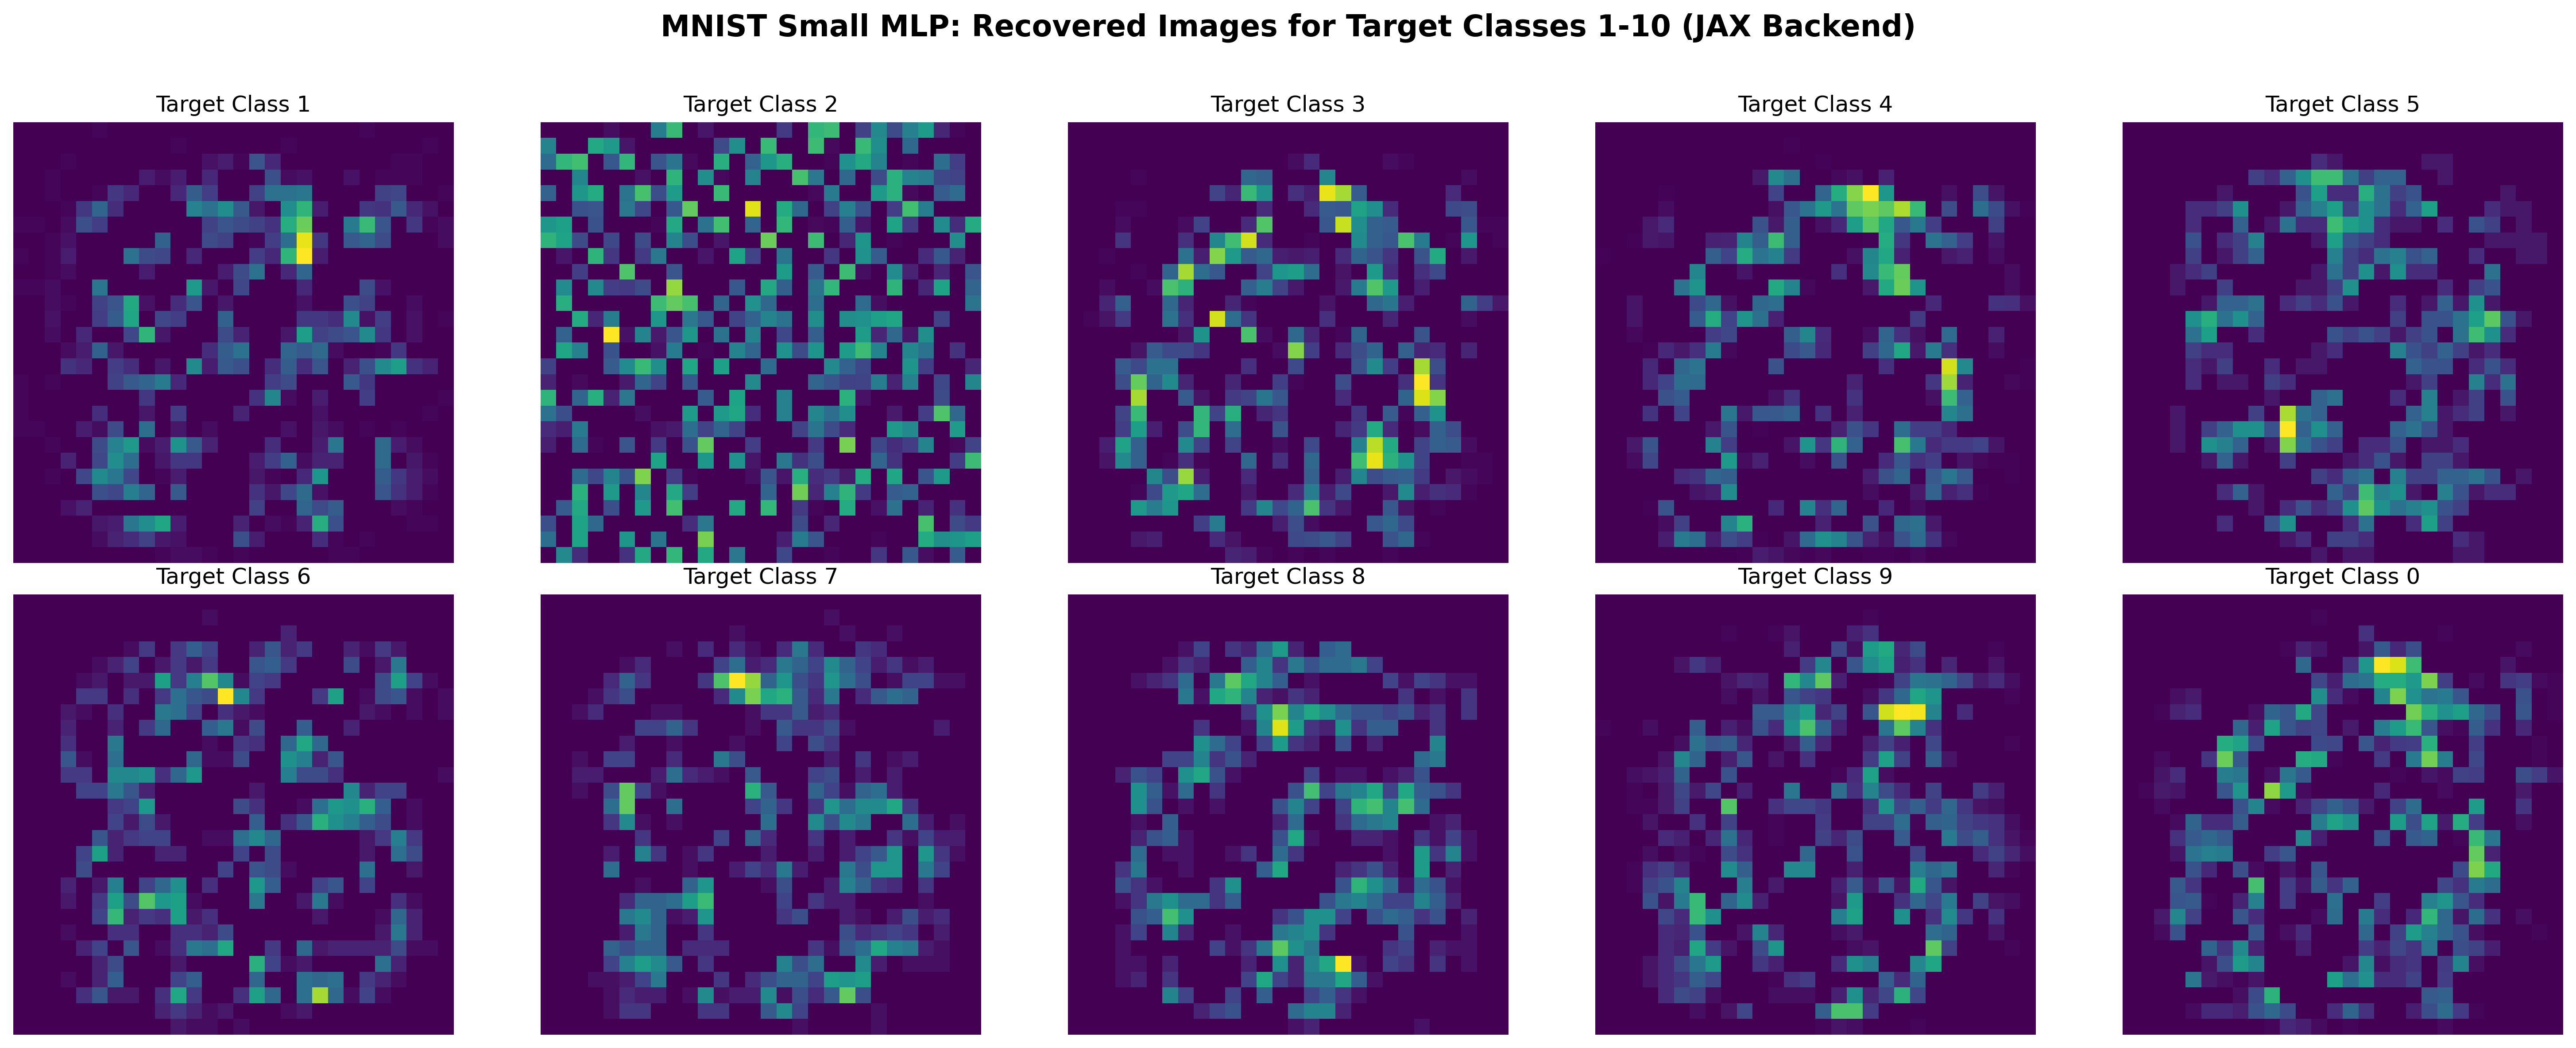
\includegraphics[width=\textwidth]{mnist_results.png}
\vspace{0.5cm}
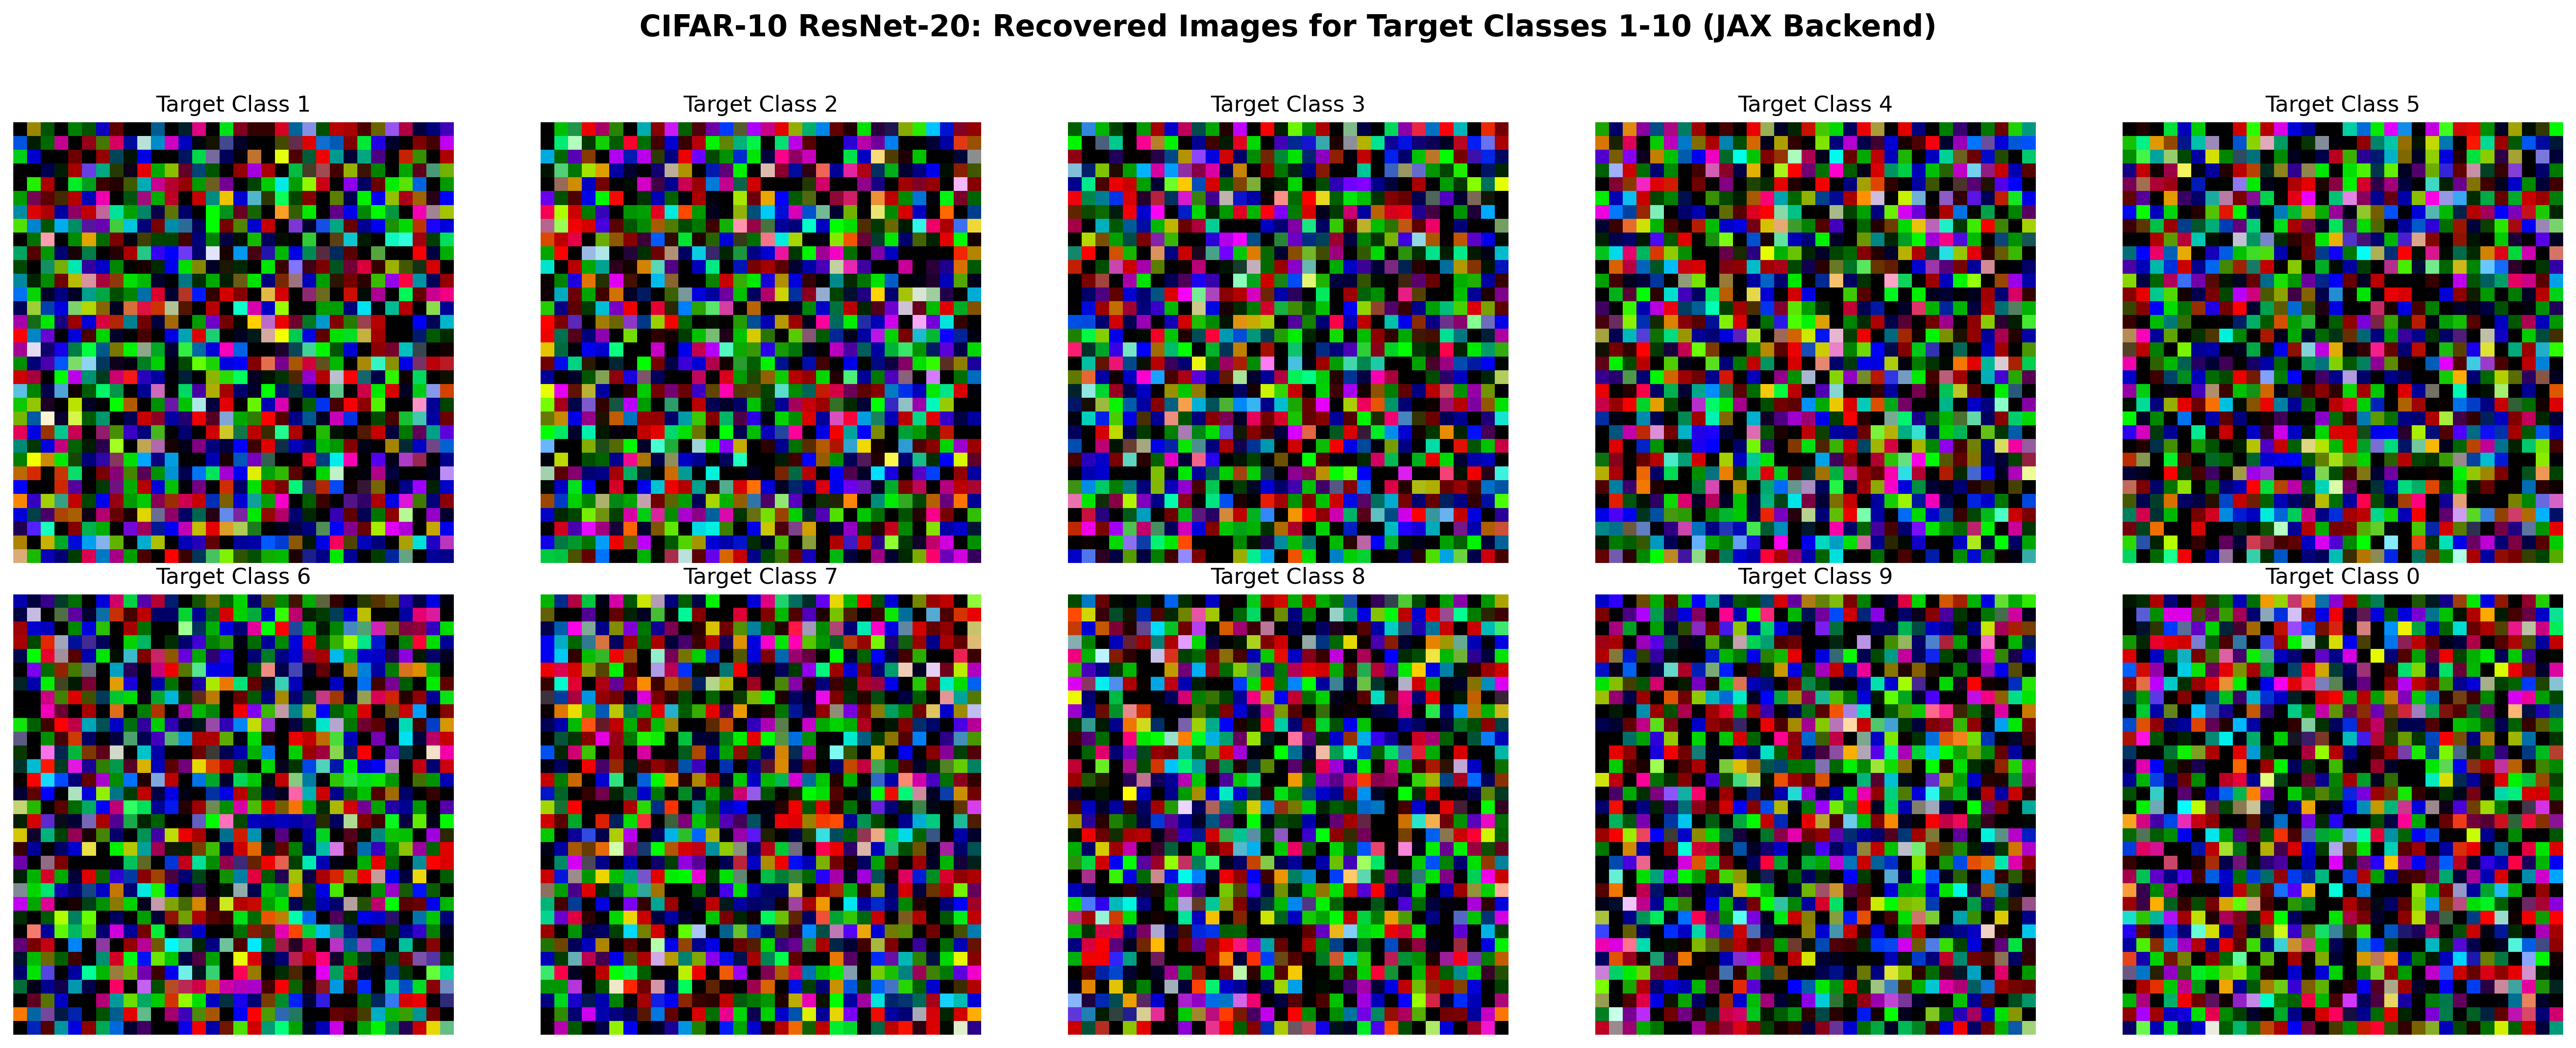
\includegraphics[width=\textwidth]{cifar_results.png}
\caption{Recovered optimal images for target classes 1--10. Top: MNIST small\_mlp model (JAX backend, 100\% success rate). Bottom: CIFAR-10 ResNet-20 model (JAX backend, 100\% success rate). Despite achieving the target class, the optimized inputs lack semantic structure and appear as noise, suggesting a high-dimensional null space in the network's input-output mapping.}
\end{figure}

\section{Interesting Ongoing Directions}

\paragraph{Systematic Benchmarking and Ablation Studies.}
The results in this report were conducted on a single CPU platform with a fixed solver configuration. A natural next step is to conduct comprehensive ablation studies across multiple dimensions:
\begin{itemize}[leftmargin=1.5em]
    \item \textbf{Hardware Platforms}: Comparing CPU performance against various GPU architectures (e.g., NVIDIA H200, Blackwell series) to quantify the benefits of GPU acceleration for both the AD backend (JAX) and the KKT linear solver (via MadNLPGPU).
    \item \textbf{Linear Solvers and KKT Formulations}: Systematically evaluating the portfolio of linear solvers available in MadNLP (e.g., HSL routines, Pardiso) and GPU-native solvers (cuDSS, cuSOLVER) in conjunction with different KKT system formulations.
    \item \textbf{Regularization and Objective Choices}: Investigating the impact of different regularization schemes (e.g., L1 for sparsity) and alternative objective functions on solver performance and solution quality.
\end{itemize}

\paragraph{Optimization on Projected Non-Convex Landscapes.}
Unlike traditional NLP problems from physical models, landscapes involving neural networks are notoriously non-convex and fragmented. Our reduced-space formulation can be interpreted as a low-dimensional projection of this high-dimensional, complex landscape onto the input decision space. If $\mathcal{L}(\theta)$ is the loss landscape over the network parameters, our objective $f(x, \mathcal{N}_\theta(x))$ is a projection where $\theta$ is fixed. The non-convexity is preserved, suggesting local solvers may find highly suboptimal solutions. This motivates exploring techniques from ML optimization, such as stochastic methods, adapted for constrained settings. More promisingly, the independence of solves for different initial points makes our framework naturally suited for \textbf{batched multi-start optimization in parallel}. This is a standard strategy for global exploration and aligns perfectly with the SIMD paradigm of GPUs.

\paragraph{Scaling to Large-Scale GPU Systems.}
To fully harness MadNLP and modern ML hardware, we must scale the problem along two axes:
\begin{enumerate}[leftmargin=1.5em]
    \item \textbf{Larger Decision Spaces ($n$)}: Current problems feature $n \sim \mathcal{O}(10^3)$. To challenge the KKT solver and further highlight MadNLP’s superiority to traditional CPU solvers, we need problems with much larger decision spaces, such as those from the control of discretized PDEs or optimizing over the latent spaces of large generative models.
    \item \textbf{Larger Neural Network Models}: The trend towards ever-larger models (e.g., Transformers) requires significant computational resources, often spanning multiple GPUs. Future work should investigate distributing the network evaluation across devices while feeding results back to a (potentially multi-GPU) MadNLP solver. This aligns our research with the core challenges of modern ML systems.
\end{enumerate}

\paragraph{Deeper Integration of ML and Optimization Ecosystems.}
Our framework serves as a bridge between the Python/JAX and Julia/MadNLP ecosystems. This could be deepened. For instance, the work by Lu et al. on embedding a first-order solver directly into JAX (\texttt{cuPDLPx.jl}) exemplifies a powerful integration pattern. We could explore similar avenues, such as creating JAX-callable wrappers for MadNLP's core routines or leveraging zero-copy data exchange between JAX and Julia on the GPU to eliminate interop overhead entirely. This would foster a more seamless environment where developers can mix and match best-in-class tools from both communities.

\paragraph{Advanced Second-Order Methods for Neural Networks.}
Building on the insight regarding efficient Hessian computation, a promising direction is the implementation of approximations that avoid forming the full Lagrangian Hessian.
\begin{itemize}[leftmargin=1.5em]
    \item \textbf{Gauss-Newton Approximation}: For objectives with small residuals at the solution ($\mathcal{N}(x^*) \approx t$), the $\sum_i r_i H_i$ term is often negligible. The Hessian can be approximated by the Gauss-Newton matrix, $J(x)^\top J(x)$, which is always positive semi-definite and computable with Jacobian-vector products.
    \item \textbf{Hessian-Vector Products}: Instead of forming the full Hessian matrix, iterative linear solvers like MINRES or GMRES only require matrix-vector products. An oracle for computing $(\nabla^2 f(x))v$ can be implemented efficiently using two backpropagation passes. Integrating this capability into MadNLP's solver options would enable second-order optimization for extremely large models where forming the Hessian explicitly is infeasible.
\end{itemize}

\section{References}
\begin{itemize}[leftmargin=1.5em]
  \item Akiba, Takuya, et al. ``Optuna: A Next-Generation Hyperparameter Optimization Framework.'' \emph{Proceedings of the 25th ACM SIGKDD International Conference on Knowledge Discovery and Data Mining}, 2019. \url{https://optuna.org}.
  \item Bradbury, James, et al. ``JAX: Composable Transformations of Python Programs.'' 2018. \url{https://github.com/google/jax}.
  \item Feder, Meir, Ruediger Urbanke, and Yaniv Fogel. ``The Universality Lens: Why Even Highly Over-Parametrized Models Learn Well.'' \emph{arXiv preprint} arXiv:2506.07661, 2025.
  \item Innes, Mike. ``Don't Unroll Adjoint: Differentiating SSA-Form Programs.'' \emph{arXiv preprint} arXiv:1810.07951, 2018. (Zygote)
  \item Innes, Mike, et al. ``Flux: Elegant Machine Learning with Julia.'' \emph{Journal of Open Source Software}, 2018. \url{https://fluxml.ai}.
  \item Lu, Haihao, et al. ``cuPDLP: A GPU-Accelerated Primal–Dual Hybrid Gradient Method for Linear Programming.'' \emph{arXiv preprint}, 2024. \url{https://github.com/cuda-mode/cuPDLP}.
  \item Lu, Haihao, et al. ``cuPDLPx.jl: Julia Interface for GPU-Accelerated PDLP.'' 2024. \url{https://github.com/JuliaConstraints/cuPDLPx.jl}.
  \item Pacaud, François, Sungho Shin, and Victor M. Zavala. ``ExaModels.jl: A Julia Modeling System for GPU-Accelerated Nonlinear Optimization.'' \emph{arXiv preprint}, 2023. \url{https://github.com/exanauts/ExaModels.jl}.
  \item Parker, Robert, et al. ``Nonlinear Optimization with GPU-Accelerated Neural Network Constraints.'' \emph{arXiv preprint} arXiv:2509.22462, 2025. \url{https://arxiv.org/pdf/2509.22462}.
  \item Paszke, Adam, et al. ``PyTorch: An Imperative Style, High-Performance Deep Learning Library.'' \emph{Advances in Neural Information Processing Systems}, 2019.
  \item Shin, Sungho, François Pacaud, and Victor M. Zavala. ``MadNLP: GPU-Accelerated Interior-Point Methods for Nonlinear Programming.'' \emph{arXiv preprint}, 2024. \url{https://github.com/MadNLP/MadNLP.jl}.
  \item Tsay, Calvin, et al. ``OMLT: Optimization and Machine Learning Toolkit.'' \emph{arXiv preprint} arXiv:2103.04751, 2021. \url{https://github.com/cog-imperial/OMLT}.
\end{itemize}
\end{document}


